% ============================================================
%  Line 2D Shape-Based Matching – Technical Documentation
%  QES (Asia-Pacific) Sdn. Bhd.
% ============================================================
\documentclass[12pt,a4paper]{article}

% ---- Encoding & fonts ----
\usepackage[T1]{fontenc}
\usepackage[utf8]{inputenc}
\usepackage{lmodern}

% ---- Page geometry ----
\usepackage[top=2.8cm, bottom=2.8cm, left=2.8cm, right=2.8cm]{geometry}

% ---- Mathematics ----
\usepackage{amsmath, amssymb, amsthm}
\usepackage{bm}

% ---- Graphics & colour ----
\usepackage{graphicx}
\usepackage{xcolor}
\usepackage{float}
\usepackage{caption}
\usepackage{subcaption}

% ---- Tables ----
\usepackage{booktabs}
\usepackage{array}
\usepackage{multirow}
\usepackage{longtable}

% ---- Code listings ----
\usepackage{listings}
\lstdefinestyle{python}{
    language=Python,
    basicstyle=\ttfamily\small,
    keywordstyle=\color{blue!80!black},
    stringstyle=\color{red!70!black},
    commentstyle=\color{green!50!black}\itshape,
    numberstyle=\tiny\color{gray},
    numbers=left,
    stepnumber=1,
    breaklines=true,
    frame=single,
    rulecolor=\color{gray!40},
    showstringspaces=false,
    tabsize=4,
}

% ---- Algorithms ----
\usepackage{algorithm}
\usepackage{algpseudocode}

% ---- Hyperlinks (load last) ----
\usepackage[
    colorlinks=true,
    linkcolor=blue!70!black,
    citecolor=blue!70!black,
    urlcolor=blue!70!black,
    bookmarks=true,
    pdfauthor={QES (Asia-Pacific) Sdn. Bhd.},
    pdftitle={Line 2D Shape Based Matching – Technical Documentation}
]{hyperref}

% ---- Headers / footers ----
\usepackage{fancyhdr}
\pagestyle{fancy}
\fancyhf{}
\lhead{\small LINE-2D Technical Documentation}
\rhead{\small QES (Asia-Pacific) Sdn.\ Bhd.}
\cfoot{\small\thepage}
\renewcommand{\headrulewidth}{0.4pt}

% ---- Section spacing ----
\usepackage{titlesec}
\titlespacing*{\section}{0pt}{2ex plus 0.5ex minus 0.2ex}{1ex plus 0.2ex}

% ---- Misc ----
\usepackage{enumitem}
\usepackage{microtype}
\usepackage{pifont}   % \ding{55} cross mark in tables

% ---- TikZ pipeline diagrams ----
\usepackage{tikz}
\usetikzlibrary{arrows.meta, positioning, fit, calc}

% ---- Helper: figure placeholder ----
\newcommand{\figplaceholder}[2]{%
  \begin{center}
    \fbox{\parbox[c][#1][c]{0.92\linewidth}{\centering\color{gray}\small[Figure placeholder: #2]}}
  \end{center}
}

% ============================================================
\begin{document}

% ---- Title page ----
\begin{titlepage}
  \centering
  \vspace*{2cm}
  {\LARGE\bfseries Line 2D Shape Based Matching\par}
  \vspace{0.6cm}
  {\large A Python Implementation of Gradient Orientation\\
           Template Matching of Wafer Alignment\par}
  \vspace{1.8cm}
  {\Huge\bfseries Technical Documentation\par}
  \vspace{2cm}
  \begin{tabular}{@{}ll@{}}
    \textbf{Algorithm:}       & Line-2D (derived from LINE-MOD)     \\[4pt]
    \textbf{References:}      & SBM\_line2D (C++ implementation)     \\[4pt]
    \textbf{Implementation:}  & Python 3.12 + OpenCV + NumPy         \\[4pt]
    \textbf{Application:}     & Wafer Fiducial Mark Detection        \\
  \end{tabular}
  \vfill
  {\large QES (Asia-Pacific) Sdn.\ Bhd.\par}
  {\large April 9, 2026\par}
\end{titlepage}

% ---- Table of contents ----
\tableofcontents
\newpage

% ============================================================
\section{Introduction}

\subsection{Background}
Template matching is a fundamental technique in machine vision for locating a known
pattern within a larger image.  Traditional methods based on pixel intensity
correlation (e.g.\ Normalized Cross-Correlation, NCC) compare raw pixel values
between a template and candidate regions of the search image.  While effective under
controlled conditions, these methods are inherently sensitive to changes in
illumination, contrast, and surface texture, because they rely directly on pixel
brightness values.

In semiconductor wafer alignment, the vision system must detect fiducial marks
(crosses, L-shapes, alignment targets) across wafers from different lots, recipes,
and process steps.  The same physical pattern can exhibit significantly different
pixel intensities depending on the wafer's surface film thickness, reflectivity, and
illumination conditions.  This makes texture-dependent methods unreliable without
frequent re-calibration.

\subsection{LINE-MOD and LINE-2D}
The LINE-MOD algorithm, introduced by Hinterstoisser, was originally designed for 3D
object detection using two modalities:
\begin{itemize}
  \item \textbf{Color Gradient Modality} --- quantized 2D edge orientations.
  \item \textbf{Depth Normal Modality} --- quantized 3D surface normals from RGB-D
        sensors.
\end{itemize}

LINE-2D is the single-modality variant that uses only the colour gradient modality,
making it suitable for standard 2D cameras without depth sensors.  The SBM
(Shape-Based Matching) LINE-2D implementation by SeanYan604 extends the original
LINE-MOD with:
\begin{itemize}
  \item Increased feature limit (up to 8191 features vs.\ the original 63).
  \item Rotation and scale invariance via template generation.
  \item Non-Maximum Suppression (NMS) for cleaner detection.
  \item Optimised single-channel (grayscale) processing.
\end{itemize}

\subsection{Key Advantage Over Texture-Based Matching}

\begin{table}[H]
  \centering
  \caption{Comparison of matching approaches}
  \label{tab:comparison}
  \begin{tabular}{lcc}
    \toprule
    \textbf{Criterion}              & \textbf{NCC}          & \textbf{LINE-2D}      \\
    \midrule
    Invariant to illumination       & No                    & Yes                   \\
    Invariant to contrast           & No                    & Yes                   \\
    Invariant to rotation           & No                    & Yes (configurable)    \\
    Invariant to scale              & No                    & Yes (configurable)    \\
    Partial occlusion tolerance     & Low                   & High                  \\
    Computational complexity        & $O(HWhw)$             & $O(HWN)$              \\
    \bottomrule
  \end{tabular}
\end{table}

% ============================================================
\section{Algorithm Overview}

The LINE-2D algorithm consists of two phases: \emph{Training} (template generation)
and \emph{Matching} (detection in search images).

\subsection{Pipeline Overview}

\begin{figure}[H]
\centering
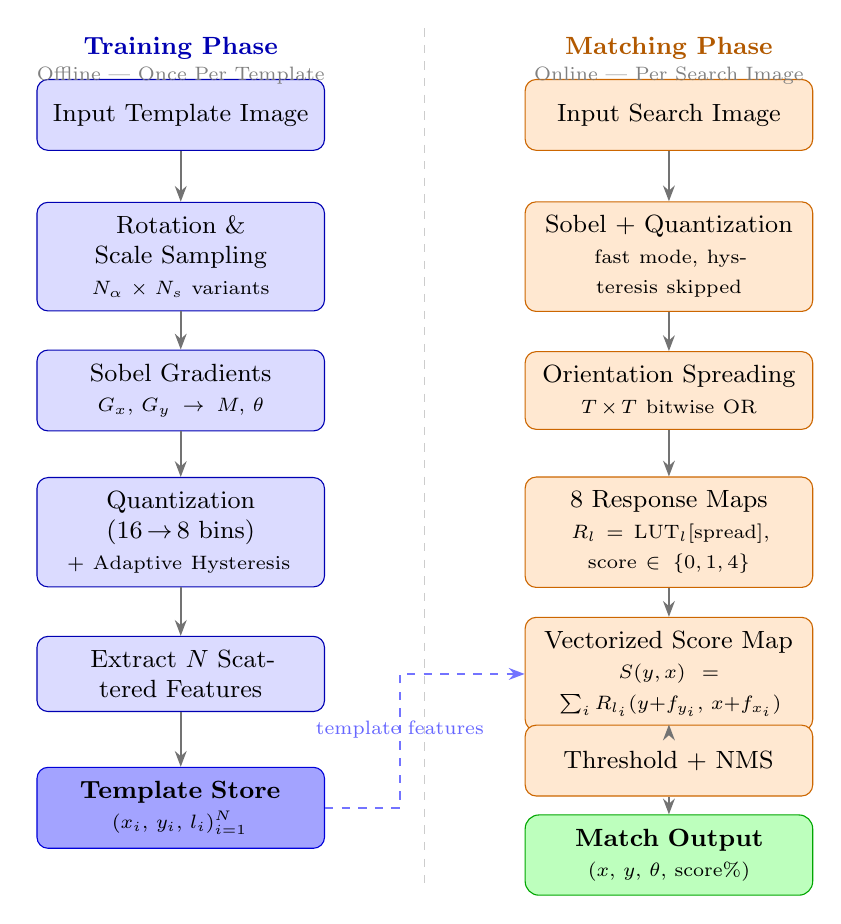
\begin{tikzpicture}[
  trainbox/.style={rectangle, rounded corners=4pt,
    draw=blue!70!black, fill=blue!14,
    text width=3.3cm, align=center,
    minimum height=0.9cm, font=\small, inner sep=5pt},
  matchbox/.style={rectangle, rounded corners=4pt,
    draw=orange!80!black, fill=orange!18,
    text width=3.3cm, align=center,
    minimum height=0.9cm, font=\small, inner sep=5pt},
  storebox/.style={rectangle, rounded corners=4pt,
    draw=blue!85!black, fill=blue!36,
    text width=3.3cm, align=center,
    minimum height=0.9cm, font=\small, inner sep=5pt},
  outbox/.style={rectangle, rounded corners=5pt,
    draw=green!65!black, fill=green!26,
    text width=3.3cm, align=center,
    minimum height=0.9cm, font=\small, inner sep=5pt},
  arr/.style={-{Stealth[length=2mm]}, thick, draw=black!55},
  darr/.style={-{Stealth[length=2mm]}, thick, draw=blue!55, dashed}
]

%% ==== Training phase ====
\node[trainbox] (T1) at (0, 0.0) {Input Template Image};
\node[trainbox] (T2) at (0,-1.8) {Rotation \& Scale Sampling\\{\scriptsize$N_\alpha \times N_s$ variants}};
\node[trainbox] (T3) at (0,-3.5) {Sobel Gradients\\{\scriptsize$G_x,\,G_y \to M,\,\theta$}};
\node[trainbox] (T4) at (0,-5.3) {Quantization (16\,$\to$\,8 bins)\\{\scriptsize + Adaptive Hysteresis}};
\node[trainbox] (T5) at (0,-7.1) {Extract $N$ Scattered Features};
\node[storebox] (T6) at (0,-8.8) {\textbf{Template Store}\\{\scriptsize$(x_i,\,y_i,\,l_i)_{i=1}^{N}$}};

%% ==== Matching phase ====
\node[matchbox] (M1) at (6.2, 0.0) {Input Search Image};
\node[matchbox] (M2) at (6.2,-1.8) {Sobel + Quantization\\{\scriptsize fast mode, hysteresis skipped}};
\node[matchbox] (M3) at (6.2,-3.5) {Orientation Spreading\\{\scriptsize$T\!\times\!T$ bitwise OR}};
\node[matchbox] (M4) at (6.2,-5.3) {8 Response Maps\\{\scriptsize$R_l=\mathrm{LUT}_l[\mathrm{spread}]$, score $\in\{0,1,4\}$}};
\node[matchbox] (M5) at (6.2,-7.1) {Vectorized Score Map\\{\scriptsize$S(y,x)=\sum_i R_{l_i}(y{+}f_{y_i},\,x{+}f_{x_i})$}};
\node[matchbox] (M6) at (6.2,-8.2) {Threshold + NMS};
\node[outbox]   (M7) at (6.2,-9.4) {\textbf{Match Output}\\{\scriptsize$(x,\,y,\,\theta,\,\mathrm{score}\%)$}};

%% ==== Training arrows ====
\foreach \a/\b in {T1/T2, T2/T3, T3/T4, T4/T5, T5/T6}
  \draw[arr] (\a)--(\b);

%% ==== Matching arrows ====
\foreach \a/\b in {M1/M2, M2/M3, M3/M4, M4/M5, M5/M6, M6/M7}
  \draw[arr] (\a)--(\b);

%% ==== Template features → Score Map ====
\draw[darr] (T6.east) -- ++(0.95,0) |-
  node[pos=0.22, above, font=\scriptsize, text=blue!60] {template features}
  (M5.west);

%% ==== Phase labels ====
\node[font=\bfseries\small, blue!70!black]    at (0,   0.85) {Training Phase};
\node[font=\scriptsize, gray]                 at (0,   0.50) {Offline --- Once Per Template};
\node[font=\bfseries\small, orange!70!black]  at (6.2, 0.85) {Matching Phase};
\node[font=\scriptsize, gray]                 at (6.2, 0.50) {Online --- Per Search Image};

%% ==== Vertical separator ====
\draw[dashed, gray!40] (3.1, 1.1) -- (3.1,-9.8);

\end{tikzpicture}
\caption{LINE-2D two-phase pipeline overview.  Training (blue, left) runs once
         offline; matching (orange, right) runs on every search image.  The dashed
         arrow shows where the stored template features are consumed during
         scoring.}
\label{fig:pipeline}
\end{figure}

\subsection{Pipeline Explanation}
The LINE-2D algorithm operates in two distinct phases, as illustrated in
Figure~\ref{fig:pipeline}.

\subsubsection{Training Phase (Offline --- Once Per Template)}
\begin{enumerate}
  \item \textbf{Input Template Image.}  A grayscale image of the fiducial mark
        (e.g.\ a cross pattern cropped from a reference wafer image).

  \item \textbf{Rotation + Scale Sampling.}  The template is rotated and scaled to
        generate $N_\alpha \times N_s$ variants.  For example, with $5^\circ$ angle
        steps and a single scale, this produces 72 template variants covering all
        possible orientations.

  \item \textbf{Sobel Gradients.}  For each variant the horizontal ($G_x$) and
        vertical ($G_y$) gradient components are computed using the Sobel operator,
        yielding the gradient magnitude $M$ and angle $\theta$ at each pixel.

  \item \textbf{Quantization (8 bins) + Hysteresis.}  The continuous angle
        $\theta \in [0^\circ, 360^\circ)$ is quantized into 8 direction bins (each
        spanning $45^\circ$), encoded as a single bit (e.g.\ bin~0 = bit~1,
        bin~3 = bit~8).  A hysteresis filter rejects weak edges
        ($M \leq T_\text{weak}$) and noise (requiring $\geq 5$ matching neighbours
        in a $3\times 3$ patch).

  \item \textbf{Extract $N$ Scattered Features.}  From the surviving edge pixels,
        $N$ spatially scattered features are selected using a greedy algorithm that
        prioritises strong edges while maintaining spatial diversity.  Each feature
        stores only $(x,\,y,\,\text{label})$ --- position and orientation bin.
\end{enumerate}

\subsubsection{Matching Phase (Online --- Per Search Image)}
\begin{enumerate}
  \item \textbf{Input Search Image.}  The full-resolution grayscale image from the
        camera in which we want to locate the fiducial mark.

  \item \textbf{Sobel + Quantization.}  Identical preprocessing as training ---
        Sobel gradients, 8-bin quantization, and hysteresis filtering are applied to
        the search image.

  \item \textbf{Orientation Spreading ($T \times T$ OR).}  The quantized
        orientations are expanded over a $T \times T$ neighbourhood using bitwise OR.
        This provides spatial tolerance: a template feature can match an edge up to
        $T$ pixels away from the exact expected position.  Since orientations are
        bit-encoded, the OR operation naturally handles multiple directions.

  \item \textbf{8 Response Maps (pre-computed from search image).}  Eight response
        maps $R_0, R_1, \ldots, R_7$ are generated from the spread image; no
        template information is used at this stage.  Each map $R_l$ answers the
        question: \emph{``If any feature with direction $l$ were placed here, what
        score would it receive?''}  Scoring uses a 256-entry Lookup Table (LUT):
        \begin{itemize}
          \item $4$ --- the spread byte at this pixel contains the exact direction
                bit (exact match).
          \item $1$ --- the spread byte contains an adjacent direction
                ($\pm 1$ bin, i.e.\ $\pm 45^\circ$).
          \item $0$ --- no matching direction is present.
        \end{itemize}

  \item \textbf{Vectorized Score Map (template used here).}  For each template
        variant, the score at every candidate position $(x,y)$ is:
        \begin{equation}
          S(y,x) = \sum_{i=1}^{N} R_{l_i}(y + f_{y_i},\; x + f_{x_i})
          \label{eq:score}
        \end{equation}
        where $(f_{x_i}, f_{y_i}, l_i)$ is the $i$-th template feature and $R_{l_i}$
        is the response map for label $l_i$.  This is normalised to a percentage:
        \begin{equation}
          \text{similarity} = \frac{S \times 100}{4N}
        \end{equation}
        Only the true fiducial mark achieves a high total score, because it is the
        only location where all $N$ features match in the correct spatial arrangement.

  \item \textbf{Threshold + NMS.}  Positions where $\text{similarity} > T_\text{match}$
        are considered candidates.  Non-Maximum Suppression (NMS) retains only the
        highest-scoring match per spatial region, suppressing nearby duplicates
        within radius $d_\text{NMS}$.
\end{enumerate}

\begin{figure}[H]
\centering
\resizebox{\textwidth}{!}{%
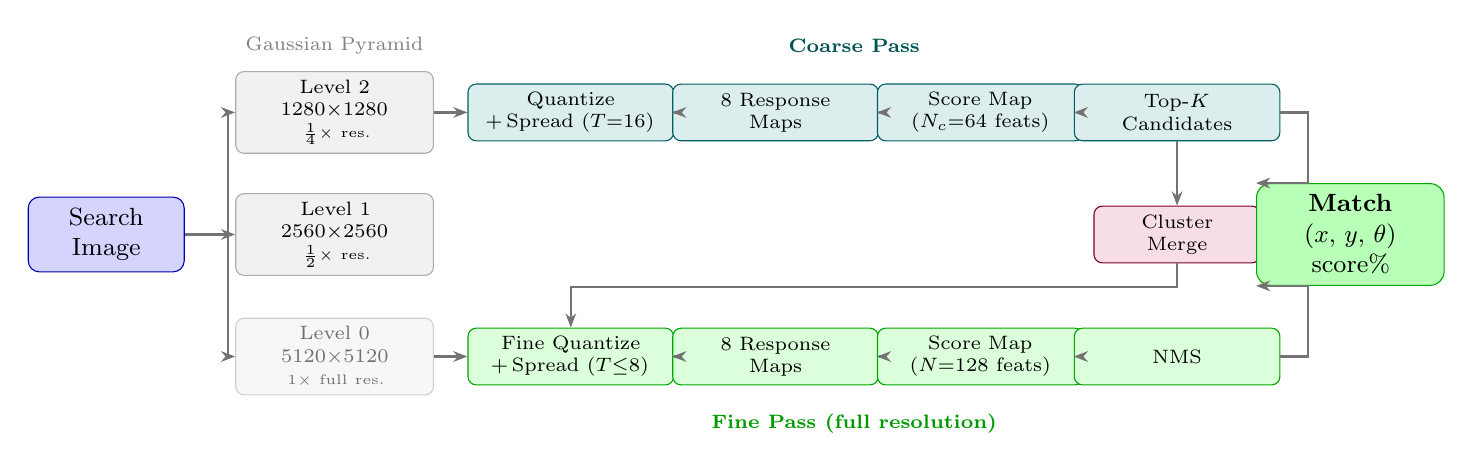
\begin{tikzpicture}[
  imgbox/.style={rectangle, rounded corners=3pt,
    draw=gray!65, fill=gray!11,
    text width=2.3cm, align=center,
    minimum height=0.72cm, font=\scriptsize, inner sep=3pt},
  cbox/.style={rectangle, rounded corners=3pt,
    draw=teal!75!black, fill=teal!14,
    text width=2.4cm, align=center,
    minimum height=0.72cm, font=\scriptsize, inner sep=3pt},
  fbox/.style={rectangle, rounded corners=3pt,
    draw=green!65!black, fill=green!14,
    text width=2.4cm, align=center,
    minimum height=0.72cm, font=\scriptsize, inner sep=3pt},
  mbox/.style={rectangle, rounded corners=3pt,
    draw=purple!65!black, fill=purple!13,
    text width=1.9cm, align=center,
    minimum height=0.72cm, font=\scriptsize, inner sep=3pt},
  outbox/.style={rectangle, rounded corners=5pt,
    draw=green!65!black, fill=green!28,
    text width=2.1cm, align=center,
    minimum height=1.1cm, font=\small, inner sep=4pt},
  arr/.style={-{Stealth[length=1.8mm]}, draw=black!55, thick},
  darr/.style={-{Stealth[length=1.8mm]}, draw=blue!55, dashed, thick}
]

%% --- Input image ---
\node[rectangle, rounded corners=4pt, draw=blue!70!black, fill=blue!17,
      text width=1.7cm, align=center, font=\small, inner sep=4pt]
  (inp) at (0,0) {Search\\Image};

%% --- Gaussian Pyramid ---
\node[font=\scriptsize, gray] at (2.9, 2.4) {Gaussian Pyramid};
\node[imgbox] (L2) at (2.9, 1.55) {Level 2\\$1280{\times}1280$\\{\tiny$\frac{1}{4}{\times}$ res.}};
\node[imgbox] (L1) at (2.9, 0.00) {Level 1\\$2560{\times}2560$\\{\tiny$\frac{1}{2}{\times}$ res.}};
\node[imgbox, opacity=0.55]
              (L0) at (2.9,-1.55) {Level 0\\$5120{\times}5120$\\{\tiny$1{\times}$ full res.}};

%% --- Coarse pass (y = 1.55) ---
\node[font=\bfseries\scriptsize, teal!65!black] at (9.5, 2.4) {Coarse Pass};
\node[cbox] (CQ)  at ( 5.9, 1.55) {Quantize\\+\,Spread ($T{=}16$)};
\node[cbox] (CRM) at ( 8.5, 1.55) {8 Response\\Maps};
\node[cbox] (CSC) at (11.1, 1.55) {Score Map\\($N_c{=}64$ feats)};
\node[cbox] (CN)  at (13.6, 1.55) {Top-$K$\\Candidates};

%% --- Cluster merge ---
\node[mbox] (CLM) at (13.6, 0.00) {Cluster\\Merge};

%% --- Fine pass (y = -1.55) ---
\node[font=\bfseries\scriptsize, green!60!black] at (9.5,-2.4) {Fine Pass (full resolution)};
\node[fbox] (FQ)  at ( 5.9,-1.55) {Fine Quantize\\+\,Spread ($T{\leq}8$)};
\node[fbox] (FRM) at ( 8.5,-1.55) {8 Response\\Maps};
\node[fbox] (FSC) at (11.1,-1.55) {Score Map\\($N{=}128$ feats)};
\node[fbox] (FN)  at (13.6,-1.55) {NMS};

%% --- Output ---
\node[outbox] (OUT) at (15.8, 0.0)
  {\textbf{Match}\\$(x,\,y,\,\theta)$\\score\%};

%% --- Input → pyramid fork ---
\draw[arr] (inp.east) -- ++(0.55,0) |- (L2.west);
\draw[arr] (inp.east) -- ++(0.55,0) |- (L1.west);
\draw[arr] (inp.east) -- ++(0.55,0) |- (L0.west);

%% --- Coarse row ---
\draw[arr] (L2)--(CQ);
\draw[arr] (CQ)--(CRM); \draw[arr] (CRM)--(CSC); \draw[arr] (CSC)--(CN);

%% --- Coarse → Cluster Merge → Fine ---
\draw[arr] (CN.south)--(CLM.north);
\draw[arr] (CLM.south) -- ++(0,-0.3) -| (FQ.north);

%% --- Fine row ---
\draw[arr] (L0)--(FQ);
\draw[arr] (FQ)--(FRM); \draw[arr] (FRM)--(FSC); \draw[arr] (FSC)--(FN);

%% --- Results → Output ---
\draw[arr] (CN.east) -- ++(0.35,0) |- (OUT.north west);
\draw[arr] (FN.east) -- ++(0.35,0) |- (OUT.south west);

\end{tikzpicture}%
}
\caption{LINE-2D coarse-to-fine pyramid pipeline (matching phase).  The coarse pass
         at $\tfrac{1}{4}$ resolution identifies candidate regions using
         $N_c = 64$ features; overlapping candidates are cluster-merged before the
         fine pass, which re-scores at full resolution ($N = 128$ features) within
         the merged ROI only.  The fine-pass spread is capped at $T \leq 8$ to
         prevent bin collisions at full resolution.}
\label{fig:pipeline_images}
\end{figure}

% ============================================================
\section{Gradient Computation and Quantization}

\subsection{Sobel Gradient Computation}
The first step computes image gradients using the Sobel operator with a $3\times 3$
kernel:
\begin{equation}
  G_x = \begin{bmatrix} -1 & 0 & 1 \\ -2 & 0 & 2 \\ -1 & 0 & 1 \end{bmatrix} * I,
  \qquad
  G_y = \begin{bmatrix} -1 & -2 & -1 \\ 0 & 0 & 0 \\ 1 & 2 & 1 \end{bmatrix} * I
\end{equation}
where $I$ is the grayscale input image and $*$ denotes 2D convolution.  The gradient
magnitude and angle are:
\begin{equation}
  M = \sqrt{G_x^2 + G_y^2},
  \qquad
  \theta = \operatorname{atan2}(G_y,\, G_x)
\end{equation}

\subsection{Orientation Quantization}
The continuous angle $\theta \in [0^\circ, 360^\circ)$ is first quantized into
16 intermediate bins, then folded into 8 direction bins by masking the lower 3
bits:
\begin{align}
  q_{16} &= \left\lfloor \theta \times \frac{16}{360} \right\rfloor \\
  q_8    &= q_{16} \;\&\; 7
\end{align}
The \texttt{\&\,7} mask folds the 16 bins symmetrically onto 8 bins, so that
opposite-direction pairs share the same label (e.g.\ a $0^\circ$ edge and a
$180^\circ$ edge both map to label~0).  This produces
$q_8 \in \{0, 1, 2, \ldots, 7\}$ where each effective bin spans $45^\circ$:

\begin{table}[H]
  \centering
  \caption{Orientation bin assignments}
  \label{tab:bins}
  \begin{tabular}{cccc}
    \toprule
    \textbf{Label $q_8$} & \textbf{Angle range}          & \textbf{Bit value} & \textbf{Direction}             \\
    \midrule
    0 & $0^\circ$--$45^\circ$    &   1 & Horizontal ($\rightarrow$)  \\
    1 & $45^\circ$--$90^\circ$   &   2 & Diagonal ($\nearrow$)       \\
    2 & $90^\circ$--$135^\circ$  &   4 & Vertical ($\uparrow$)       \\
    3 & $135^\circ$--$180^\circ$ &   8 & Diagonal ($\nwarrow$)       \\
    4 & $180^\circ$--$225^\circ$ &  16 & Horizontal ($\leftarrow$)   \\
    5 & $225^\circ$--$270^\circ$ &  32 & Diagonal ($\swarrow$)       \\
    6 & $270^\circ$--$315^\circ$ &  64 & Vertical ($\downarrow$)     \\
    7 & $315^\circ$--$360^\circ$ & 128 & Diagonal ($\searrow$)       \\
    \bottomrule
  \end{tabular}
\end{table}

The label is encoded as a single bit:
\begin{equation}
  \text{quantized}(x,y) = 2^{\,q_8}
\end{equation}
This bit encoding is critical for the spreading and response map steps.

\subsection{Hysteresis Filtering}
To suppress noise and ensure spatial consistency, a hysteresis filter is applied.
For each pixel $(x,y)$:
\begin{enumerate}
  \item \textbf{Magnitude threshold.}  Reject pixels where
        $M(x,y) \leq T_\text{weak}$.  When \texttt{WEAK\_THRESHOLD} is negative,
        its absolute value is treated as a percentile of all non-zero gradient
        magnitudes in the image (e.g.\ the default value $-70$ uses the adaptive
        70th-percentile threshold rather than a fixed constant).

  \item \textbf{Adaptive neighbourhood majority vote.}  The voting kernel size
        $k_s$ is resolved \emph{once} from the full image's longest dimension
        before any pyramid passes:
        \begin{equation}
          k_s = \min\!\bigl(\text{raw\_ks} \mid_{\text{odd}},\; 9\bigr)
        \end{equation}
        where $|\cdot|_\text{odd}$ denotes rounding up to the nearest odd integer.
        The required vote count is:
        \begin{equation}
          V_\text{min} = \left\lfloor k_s^2 / 2 \right\rfloor + 1
        \end{equation}
        At $k_s = 3$ this gives $V_\text{min} = 5$ (classic behaviour); at
        $k_s = 9$ it gives $V_\text{min} = 41$.  A pixel is accepted only when its
        dominant label~$q^*$ receives $\geq V_\text{min}$ votes in the
        $k_s \times k_s$ neighbourhood:
        \begin{equation}
          q^* = \arg\max_k \operatorname{hist}(k)
          \quad\text{over the } k_s \times k_s \text{ patch}
        \end{equation}
\end{enumerate}

\subsubsection{Vectorized Implementation}
The na\"ive Python loop is prohibitively slow ($O(H \times W)$ iterations).
The vectorized implementation processes all pixels simultaneously:
\begin{enumerate}
  \item Build 8 binary planes: $P_i(x,y) = \mathbf{1}[q_8(x,y) = i]$ for
        $i = 0, \ldots, 7$.
  \item Apply \texttt{cv2.filter2D} (\texttt{CV\_16U} output depth) with a
        $k_s \times k_s$ all-ones kernel to each plane, producing per-bin vote
        counts $V_i$.
  \item Track the per-pixel winner via a running \texttt{best\_label} /
        \texttt{best\_count} comparison (\texttt{votes > best\_count}), which
        avoids a full \texttt{np.argmax} call and is marginally faster.
  \item Accept pixels where $M > T_\text{weak}$ and $V^* \geq V_\text{min}$.
\end{enumerate}
This reduces computation from $\sim$14 seconds to $\sim$13\,ms for a
$1080\times 1080$ image.

\subsection{GPU-Accelerated Gradient Path}
\label{sec:cuda}

When an NVIDIA GPU is available (\texttt{cv2.cuda} is importable and at least one
CUDA-capable device is present), the computationally heavy Blur + Sobel + Magnitude
+ Angle operations are offloaded to the GPU via OpenCV's \texttt{cv2.cuda} module.
This reduces the latency of the gradient step on large $5120 \times 5120$ sensor
images from $\sim$80\,ms (CPU) to $\sim$15\,ms (GPU).

\subsubsection{Detection at Import Time}
CUDA availability is probed \emph{once} at module import time to avoid repeated
runtime checks:

\begin{lstlisting}[style=python, caption={One-shot CUDA detection at import},
                   label={lst:cuda_detect}]
try:
    _CUDA_DEVICE_COUNT = cv2.cuda.getCudaEnabledDeviceCount()
except Exception:
    _CUDA_DEVICE_COUNT = 0
_CUDA_AVAILABLE = _CUDA_DEVICE_COUNT > 0
\end{lstlisting}

The result is stored in module-level constants \texttt{\_CUDA\_AVAILABLE} and
\texttt{\_CUDA\_DEVICE\_COUNT}.  \texttt{LinemodConfig.USE\_GPU} is initialised to
\texttt{\_CUDA\_AVAILABLE} automatically so the GPU path is enabled by default
when hardware is present and can be overridden by setting \texttt{cfg.USE\_GPU = False}.

\subsubsection{GPU Operations Performed}
The following operations run on the GPU when \texttt{use\_gpu=True}:

\begin{enumerate}
  \item \textbf{Upload.}  The \texttt{float32} grayscale array is uploaded to a
        \texttt{cv2.cuda\_GpuMat} via \texttt{gpu\_gray.upload(gray)}.

  \item \textbf{Gaussian blur (conditional).}  Applied only during the
        \emph{template training} pass (\texttt{fast\_mode=False}).  The sigma
        and kernel size are computed adaptively from the image's longest dimension
        (same formula as the CPU path):
        \begin{equation}
          \sigma = \max\!\bigl(1.0,\; \tfrac{d_\text{max} - 1000}{1500}\bigr),
          \qquad
          k = 2\lfloor\sigma\rfloor + 1
        \end{equation}
        A \texttt{cv2.cuda.createGaussianFilter} filter object is constructed and
        applied via \texttt{.apply()}.

  \item \textbf{Sobel gradients.}  $G_x$ and $G_y$ are computed via two
        \texttt{cv2.cuda.createSobelFilter} objects (\texttt{ksize=3},
        \texttt{dtype=CV\_32F}), producing two \texttt{GpuMat} buffers that remain
        on-device.

  \item \textbf{Magnitude and angle.}
        \begin{align}
          M   &= \texttt{cv2.cuda.magnitude}(G_x, G_y) \\
          \phi &= \texttt{cv2.cuda.phase}(G_x, G_y,\;\texttt{angleInDegrees=True})
        \end{align}
        Both results are \texttt{GpuMat} buffers.

  \item \textbf{Selective download.}  Only \texttt{magnitude} and \texttt{angle}
        are downloaded to host memory (\texttt{.download()}).  The intermediate
        buffers $G_x$, $G_y$, and the blurred \texttt{gpu\_gray} are kept on-device
        until Python's garbage collector releases them, avoiding two unnecessary
        large PCIe transfers.
\end{enumerate}

After download, all remaining steps (quantization, hysteresis majority vote) execute
on the CPU using the downloaded arrays, exactly as in the CPU-only path.

\subsubsection{GPU Code Listing}

\begin{lstlisting}[style=python,
  caption={GPU path inside \texttt{\_quantize\_gradients()}},
  label={lst:cuda_path}]
if use_gpu and _CUDA_AVAILABLE:
    try:
        gpu_gray = cv2.cuda_GpuMat()
        gpu_gray.upload(gray)                          # (1) Upload

        if not fast_mode:                              # (2) Blur (training only)
            sigma = max(1.0, (max_dim - 1000) / 1500.0)
            ksize = int(sigma * 2) * 2 + 1
            blur = cv2.cuda.createGaussianFilter(
                cv2.CV_32F, cv2.CV_32F, (ksize, ksize), sigma)
            gpu_gray = blur.apply(gpu_gray)

        sobel_x = cv2.cuda.createSobelFilter(          # (3) Sobel
            cv2.CV_32F, cv2.CV_32F, 1, 0, ksize=3)
        sobel_y = cv2.cuda.createSobelFilter(
            cv2.CV_32F, cv2.CV_32F, 0, 1, ksize=3)
        gpu_dx = sobel_x.apply(gpu_gray)
        gpu_dy = sobel_y.apply(gpu_gray)

        gpu_mag   = cv2.cuda.magnitude(gpu_dx, gpu_dy, # (4) Magnitude & angle
                        cv2.cuda_GpuMat())
        gpu_angle = cv2.cuda.phase(gpu_dx, gpu_dy,
                        cv2.cuda_GpuMat(), angleInDegrees=True)

        magnitude = gpu_mag.download()                 # (5) Selective download
        angle     = gpu_angle.download() % 360.0
        _did_gpu  = True
    except Exception as e:
        print(f"[LINE-2D CUDA ERROR] Fallback to CPU: {e}")
        _did_gpu = False
\end{lstlisting}

\subsubsection{Graceful CPU Fallback}
The entire GPU block is wrapped in a \texttt{try/except}.  Any CUDA error ---
out-of-memory, unsupported operation, driver mismatch --- is caught silently and the
flag \texttt{\_did\_gpu} remains \texttt{False}, causing the code to fall through to
the identical CPU path.  This means the matcher never crashes due to a GPU error;
it simply runs slightly slower.

\subsubsection{Where GPU Is \emph{Not} Used}
\label{sec:cuda_exclusions}

Not every step benefits from GPU acceleration.  The following calls explicitly pass
\texttt{use\_gpu=False}:

\begin{table}[H]
  \centering
  \caption{GPU usage decisions per pipeline stage}
  \label{tab:cuda_decisions}
  \begin{tabular}{p{5.5cm}lp{5.8cm}}
    \toprule
    \textbf{Stage}                      & \textbf{GPU?} & \textbf{Reason}             \\
    \midrule
    Template training quantize          & \checkmark    & Large image, non-realtime, benefits from parallelism \\
    Single-level search quantize        & \checkmark    & Full-resolution $5120^2$ image \\
    Coarse pyramid quantize             & \ding{55}     & Image is $\tfrac{1}{4}$ downsampled ($\sim$1280\,px); PCIe round-trip overhead exceeds GPU compute saving \\
    Fine-pass (ROI) quantize            & \ding{55}     & ROI is typically $200$--$400$\,px; host $\leftrightarrow$ device transfer would dominate \\
    Spread (\texttt{\_spread})          & \ding{55}     & 8 separate bit-plane \texttt{cv2.dilate} calls; CPU SIMD is faster than PCIe cost for small planes \\
    \bottomrule
  \end{tabular}
\end{table}

The key PCIe trade-off: for a $5120 \times 5120$ \texttt{float32} image the upload
is $\approx 100\,\text{MB}$; at PCIe~3.0 $\times16$ bandwidth ($12\,\text{GB/s}$)
this costs $\approx 8\,\text{ms}$.  The GPU Sobel + magnitude on that image takes
$\approx 2\,\text{ms}$.  The combined GPU path ($\approx 10\,\text{ms}$ including
download) beats the CPU path ($\approx 80\,\text{ms}$) by $8\times$.  For a
$400 \times 400$ ROI the upload is $0.6\,\text{MB}$ ($< 0.1\,\text{ms}$), the CPU
Sobel takes $< 1\,\text{ms}$, so batching to GPU would have negative ROI.

\subsubsection{Requirements}
\begin{itemize}
  \item \textbf{NVIDIA GPU} with CUDA Compute Capability $\geq 3.5$.
  \item \textbf{OpenCV built with CUDA support} ---
        \texttt{opencv-contrib-python} from PyPI does \emph{not} include CUDA.
        A custom build or a pre-built CUDA wheel (e.g.\
        \texttt{opencv-python-cuda}) is required.
  \item \textbf{CUDA Toolkit} matching the OpenCV build version installed on the
        host machine.
\end{itemize}
If any of the above is absent, \texttt{cv2.cuda.getCudaEnabledDeviceCount()}
raises an \texttt{AttributeError} which is caught at import time and
\texttt{\_CUDA\_AVAILABLE} is set to \texttt{False}; the matcher operates purely
on the CPU path without any code change.

\subsection{Fast Mode --- Hysteresis Skip}
During the \emph{matching phase}, the search image must be quantized once per
detection request.  Because the hysteresis $k_s \times k_s$ majority-vote is
relatively expensive and the spatial spreading step (§\ref{sec:spreading_alg})
already provides tolerance for noisy quantization, the implementation supports
\texttt{FAST\_SEARCH\_QUANTIZE = True} (enabled by default).  In fast mode the
majority-vote step is skipped entirely; only the magnitude threshold
$M > T_\text{weak}$ is applied.  This gives a significant speed gain on large
search images with negligible impact on detection accuracy.

% ============================================================
\section{Orientation Spreading}

\subsection{Purpose}
The spreading operation adds spatial tolerance to the quantized orientations.
Without spreading, a feature must land at the exact pixel position of the
corresponding edge in the search image.  With spreading parameter $T$, the feature
can be up to $T$ pixels away and still match.

\subsection{Algorithm}
\label{sec:spreading_alg}
The spreading operation applies a bitwise OR over a $T \times T$ neighbourhood:
\begin{equation}
  \text{spread}(x,y)
  = \bigvee_{(dx,\,dy)\;\in\;
             \bigl[-\lfloor T/2\rfloor,\,\lfloor T/2\rfloor\bigr]^{2}}
    Q(x+dx,\;y+dy)
\end{equation}
where $Q$ is the quantized image and $\vee$ denotes bitwise OR.  Since each label is
encoded as a distinct bit, OR-ing multiple labels produces a byte where multiple bits
can be set, indicating that multiple orientations are present within the
$T \times T$ neighbourhood.

\textbf{Example.}  If $T=4$ and a pixel has a horizontal edge (label~$=0$,
bit~$=1$) while its neighbour 3 pixels away has a vertical edge (label~$=2$,
bit~$=4$), the spread result at their overlap is
$1 \vee 4 = 5 = \texttt{0b00000101}$, indicating both orientations are present.

\subsection{Implementation}
The spreading is implemented by applying \texttt{cv2.dilate} independently to
each of the 8 bit-planes extracted from the quantized image, using a square
structuring element of size $T \times T$:

\begin{lstlisting}[style=python, caption={Bit-plane dilation spreading}]
spread = np.zeros_like(quantized)
struct = cv2.getStructuringElement(cv2.MORPH_RECT, (T, T))
for bit in range(8):
    plane = ((quantized >> bit) & 1).astype(np.uint8) * 255
    dilated = cv2.dilate(plane, struct)
    spread |= ((dilated > 0).astype(np.uint8) << bit)
\end{lstlisting}

This is mathematically equivalent to the two-pass horizontal/vertical OR
formulation in~§\ref{sec:spreading_alg}, but exploits OpenCV's highly optimised
morphological dilation path.  The result is the same spread byte
$\text{spread}(x,y)$ described in §\ref{sec:spreading_alg}.

% ============================================================
\section{Response Map Computation}

\subsection{Lookup Table Design}
For each of the 8 possible template labels, a 256-entry Lookup Table (LUT) maps the
spread byte at a search image position to a similarity score:
\begin{equation}
  \text{LUT}_l[v] =
  \begin{cases}
    4 & \text{if bit } l \text{ is set in } v \quad (\text{exact match}) \\
    1 & \text{if an adjacent direction bit is set in } v \\
    0 & \text{otherwise}
  \end{cases}
\end{equation}
where $l \in \{0,1,\ldots,7\}$ is the template feature label and
$v \in \{0,1,\ldots,255\}$ is the spread byte value.

\begin{table}[H]
  \centering
  \caption{Example LUT entries for label $l = 2$
           (angle bin $90^\circ$--$135^\circ$, bit~4)}
  \label{tab:lut}
  \begin{tabular}{ccl}
    \toprule
    \textbf{Spread byte $v$} & \textbf{Binary}          & \textbf{Score} \\
    \midrule
    4   & \texttt{0000\,0100} & 4 (exact match)          \\
    2   & \texttt{0000\,0010} & 1 (adjacent, bin~1)      \\
    8   & \texttt{0000\,1000} & 1 (adjacent, bin~3)      \\
    6   & \texttt{0000\,0110} & 4 (exact $+$ adjacent)   \\
    1   & \texttt{0000\,0001} & 0 (no match)             \\
    255 & \texttt{1111\,1111} & 4 (all bits set)         \\
    \bottomrule
  \end{tabular}
\end{table}

\subsection{Response Map Generation}
Eight response maps $R_0, R_1, \ldots, R_7$ are computed by applying each LUT to the
spread image:
\begin{equation}
  R_l(x,y) = \text{LUT}_l\bigl[\text{spread}(x,y)\bigr],
  \quad l = 0, 1, \ldots, 7
\end{equation}
This is a simple table lookup: each pixel of the spread image indexes into the
256-entry LUT, producing a score in $\{0, 1, 4\}$.

% ============================================================
\section{Sparse Feature Extraction}

\subsection{Motivation}
Rather than storing and comparing the entire quantized template image, LINE-2D
selects a small number of spatially scattered feature points ($N$, typically
64--128).  This provides two key advantages:
\begin{itemize}
  \item \textbf{Speed.} Scoring requires only $N$ lookups per candidate position,
        rather than a full-image convolution.
  \item \textbf{Robustness.} Sparse sampling tolerates partial occlusion --- if $M$
        out of $N$ features match, the object is still detected with score $M/N$.
\end{itemize}

\subsection{Selection Algorithm}
The feature selection follows a greedy scattered sampling approach with an
\emph{adaptive} initial separation distance that scales with the template size:
\begin{enumerate}
  \item Sort all surviving edge pixels by gradient magnitude (descending).
  \item Compute the initial minimum separation from the template bounding box:
        \begin{equation}
          d_0 = \frac{2\,(W_t + H_t)}{N \times 0.8}
        \end{equation}
        where $W_t, H_t$ are the template dimensions.
  \item Initialise an empty feature set $\mathcal{F} = \emptyset$ and a boolean
        \texttt{used[]} bitmask of length $C$ (number of candidate pixels).
  \item \textbf{Distance-relaxation loop.}  While $|\mathcal{F}| < N$ and $d > 1$:
        \begin{enumerate}
          \item For each \emph{un-used} candidate $(x,y)$ in sorted order:
                accept if $\|(x,y)-(x',y')\|_2^2 \geq d^2$ for all
                $(x',y') \in \mathcal{F}$; mark candidate \texttt{used}.
          \item Relax: $d \leftarrow d - \max\!\bigl(1.0,\; d \times 0.15\bigr)$.
        \end{enumerate}
\end{enumerate}
Each feature stores only three values: $(x, y, \text{label})$ --- position relative
to the template origin and quantized orientation bin.

\textbf{Implementation notes.}
The minimum-distance check is fully vectorized using pre-allocated NumPy arrays,
avoiding any inner Python loop over accepted features:
\begin{lstlisting}[style=python, caption={Vectorized minimum-distance check}]
dists = (fxs[:n_kept] - x)**2 + (fys[:n_kept] - y)**2
if not np.any(dists < dist_sq):
    fxs[n_kept] = x;  fys[n_kept] = y;  n_kept += 1
\end{lstlisting}
The \texttt{used[]} bitmask prevents the same candidate from being re-evaluated
across relaxation passes, keeping each pass $O(C)$ regardless of the number of
features already accepted.

\subsection{Template Cropping}
After feature extraction, \texttt{cropTemplates()} computes the tight bounding box
of all features and makes positions relative to it:
\begin{align}
  tl_x &= \min_i f_{x_i}, \quad tl_y = \min_i f_{y_i} \\
  br_x &= \max_i f_{x_i}, \quad br_y = \max_i f_{y_i}
\end{align}
Feature positions are then adjusted:
$f_{x_i} \leftarrow f_{x_i} - tl_x$,\; $f_{y_i} \leftarrow f_{y_i} - tl_y$.

% ============================================================
\section{Template Generation}

\subsection{Rotation and Scale Sampling}
To achieve rotation and scale invariance, the algorithm generates multiple template
variants by transforming the original template image:
\begin{equation}
  I_{\alpha,s} = W_{\alpha,s}(I_0)
\end{equation}
where $W$ applies rotation by angle $\alpha$ and uniform scaling by factor $s$ around
the template centre using bilinear interpolation:
\begin{equation}
  W_{\alpha,s} = s\cdot\begin{bmatrix} \cos\alpha & -\sin\alpha \\
                                        \sin\alpha &  \cos\alpha \end{bmatrix}
\end{equation}

\subsection{Configuration Parameters}

\begin{table}[H]
  \centering
  \caption{Full configuration parameters (\texttt{LinemodConfig})}
  \label{tab:params}
  \begin{tabular}{p{5.2cm}p{3.2cm}p{5.5cm}}
    \toprule
    \textbf{Parameter}                    & \textbf{Default}            & \textbf{Description}                                                \\
    \midrule
    \texttt{ANGLE\_STEP}                  & $5^\circ$                   & Angular increment for rotation sampling                             \\
    \texttt{ANGLE\_START}                 & $0^\circ$                   & Starting angle                                                      \\
    \texttt{ANGLE\_END}                   & $360^\circ$                 & Ending angle                                                        \\
    \texttt{SCALE\_MIN}                   & $1.0$                       & Minimum scale factor                                                \\
    \texttt{SCALE\_MAX}                   & $1.0$                       & Maximum scale factor                                                \\
    \texttt{SCALE\_STEP}                  & $0.1$                       & Scale increment                                                     \\
    \texttt{NUM\_FEATURES} ($N$)          & $128$                       & Features per template variant                                       \\
    \texttt{WEAK\_THRESHOLD}              & $-70.0$                     & Gradient threshold; negative value = adaptive $n$-th percentile
                                                                         of non-zero magnitudes (e.g.\ $-70$ $\Rightarrow$ 70th percentile) \\
    \texttt{T\_PYRAMID}                   & $[4,\,8,\,16]$              & Spread radius per pyramid level (fine to coarse)                    \\
    \texttt{PYRAMID\_LEVELS}$^\dagger$    & \texttt{len(T\_PYRAMID)}    & Read-only property; number of active pyramid levels                 \\
    \texttt{NMS\_DISTANCE}                & $10$                        & Min pixel distance between kept matches (NMS radius)                \\
    \texttt{COARSE\_NUM\_FEATURES}        & $64$                        & Features used during coarse pyramid scoring                         \\
    \texttt{MAX\_COARSE\_CANDIDATES}      & $20$                        & Max candidates forwarded from coarse to fine pass                   \\
    \texttt{FAST\_SEARCH\_QUANTIZE}       & \texttt{True}               & Skip hysteresis on search image (fast mode, see §3.5)               \\
    \bottomrule
  \end{tabular}
\end{table}
{\small $^\dagger$~\texttt{PYRAMID\_LEVELS} is a \texttt{@property} derived from
\texttt{len(T\_PYRAMID)}; it cannot be set directly.}

Total templates generated: $N_\alpha \times N_s$ where
$N_\alpha = \lfloor 360/\texttt{ANGLE\_STEP}\rfloor$ and
$N_s = \lfloor(\text{SCALE\_MAX} - \text{SCALE\_MIN})/\text{SCALE\_STEP}\rfloor + 1$.

\subsection{Region of Interest (ROI) Masking}
To maximise matching robustness and completely eliminate background noise, the
template generation pipeline incorporates a user-defined Region of Interest (ROI)
masking feature.  A standard rectangular bounding box often captures irrelevant
background textures or adjacent structures that can degrade matching accuracy and
create false-positive features.

The ROI masking tool allows the user to explicitly ``paint'' over the critical
structural features of the target pattern (such as the distinct outline of a
cross-shaped fiducial).  This process generates a binary mask $M$ with the same
dimensions as the extracted bounding box $I_\text{ROI}$:
\begin{equation}
  M(x,y) =
  \begin{cases}
    1 & \text{if pixel } (x,y) \text{ lies within the painted ROI} \\
    0 & \text{otherwise}
  \end{cases}
\end{equation}
During the feature extraction phase, the algorithm only computes gradients and
records features at coordinates where $M(x,y) = 1$.  By ignoring all unmasked
regions, the generated template strictly represents the intended geometry, making the
matcher highly invariant to variations in the surrounding background context.

% ============================================================
\section{Matching: Vectorized Response Map Scoring}

\subsection{Score Map Construction}
The matching phase computes a similarity score map $S(y,x)$ for each template.  At
every candidate position $(x,y)$, the score is the sum of response values at each
feature's offset:
\begin{equation}
  S(y,x) = \sum_{i=1}^{N} R_{l_i}(y + f_{y_i},\; x + f_{x_i})
\end{equation}
where $(f_{x_i}, f_{y_i}, l_i)$ is the $i$-th template feature and $R_{l_i}$ is the
response map for label $l_i$.

\subsection{Vectorized Implementation}
Rather than iterating over every $(x,y)$ position in Python, we exploit NumPy's
array slicing:

\begin{lstlisting}[style=python, caption={Vectorized score map accumulation}]
score_map = np.zeros((H - h, W - w), dtype=np.float32)
for fx, fy, label in features:
    score_map += response_maps[label][fy : fy + (H - h),
                                      fx : fx + (W - w)]
\end{lstlisting}

Each feature contributes a single NumPy array addition of a shifted slice of its
corresponding response map.  The total computation performs $N$ array additions
(typically $N = 64$ or $128$), regardless of image size.  This achieves
$O(H \cdot W \cdot N)$ complexity --- asymptotically equal to the na\"ive Python loop
implementation, but $\sim 100\times$ faster in practice due to NumPy's C-level inner
loop.  Note: the timing figures cited in earlier versions of this document
($\sim$375\,ms Python vs $\sim$5\,ms C++ for a $1080\times 1080$ image) predate the
pyramid strategy described in §12; with the coarse-to-fine pyramid the effective
search area at full resolution is much smaller and total wall-clock time is well
under 2 seconds on $5120\times 5120$ images.

\subsection{Score Normalization}
The raw score is normalized to a percentage:
\begin{equation}
  \text{similarity}(y,x) = \frac{S(y,x)}{4 \times N} \times 100\%
\end{equation}
The denominator $4 \times N$ is the maximum possible score when all $N$ features
achieve an exact match (score 4 each).

\subsection{Comparison with C++ Linearized Memory}
The original C++ implementation uses a linearized memory data structure to optimize
memory access patterns for SIMD (SSE2) processing.  Each response map is decimated
into $T \times T$ sub-grids stored as contiguous memory rows, enabling sequential
access during scoring.

In Python, this optimization is counterproductive --- Python loop overhead dominates
any memory-access benefit.  Our NumPy array-slicing approach is equivalent in
result but leverages Python's strengths:

\begin{table}[H]
  \centering
  \caption{Scoring approach comparison}
  \label{tab:scoring}
  \begin{tabular}{lll}
    \toprule
    \textbf{Aspect}        & \textbf{C++ Linearized Memory} & \textbf{Python NumPy}        \\
    \midrule
    Memory layout          & Row-major, decimated           & Standard 2-D array           \\
    Parallelism            & SIMD (SSE2)                    & NumPy C-level BLAS           \\
    Loop overhead          & Minimal                        & Eliminated by vectorization  \\
    Cache optimization     & Explicit                       & Implicit (contiguous slices) \\
    \bottomrule
  \end{tabular}
\end{table}

% ============================================================
\section{Post-Processing}

\subsection{Thresholding}
Candidate matches are extracted where $\text{similarity}(y,x) > T_\text{match}$.
The threshold $T_\text{match}$ (default 50\%) controls the trade-off between
detection sensitivity and false positive rate.

\subsection{Non-Maximum Suppression (NMS)}
Multiple above-threshold positions typically cluster around the true match location
due to the spreading tolerance.  NMS retains only the strongest match per spatial
region:
\begin{enumerate}
  \item Sort all candidate positions by score (descending).
  \item For each candidate $(x,y)$ in sorted order:
        \begin{enumerate}
          \item If no accepted match exists within distance $d_\text{NMS}$, accept
                $(x,y)$.
          \item Otherwise, suppress it.
        \end{enumerate}
\end{enumerate}

\subsection{Match Position Computation}
The final match position is computed as the centre of the template image at the
detected location:
\begin{align}
  x_\text{match} &= x_\text{scan} + tl_x + \frac{W_\text{template}}{2} \\
  y_\text{match} &= y_\text{scan} + tl_y + \frac{H_\text{template}}{2}
\end{align}
where $(x_\text{scan}, y_\text{scan})$ is the position in the score map,
$(tl_x, tl_y)$ is the feature bounding box offset, and
$(W_\text{template}, H_\text{template})$ is the original template image size.

% ============================================================
\section{Implementation Details}

\subsection{Class and Function Structure}
\begin{itemize}
  \item \texttt{LinemodConfig} --- Configuration dataclass with all parameters.
  \item \texttt{Feature} --- Struct: $(x, y, \text{label})$.
  \item \texttt{TemplatePyr} --- Per-level template: Feature $+$ Bounding Box.
  \item \texttt{LinemodMatcher} --- Main class:
        \texttt{load\_template()}, \texttt{generate\_templates()}, \texttt{match()}.
  \item \texttt{quantize\_gradients()} --- Sobel $+$ quantization $+$ hysteresis.
  \item \texttt{\_spread()} --- $T \times T$ OR spreading.
  \item \texttt{\_compute\_response\_maps()} --- LUT-based response maps.
  \item \texttt{\_extract\_scattered\_features()} --- Greedy feature selection.
  \item \texttt{\_crop\_template()} --- Bounding box normalization.
  \item \texttt{\_subpixel\_refine()} --- Parabolic sub-pixel interpolation (§\ref{sec:subpixel}).
\end{itemize}

\subsection{Usage Example}

\begin{lstlisting}[style=python, caption={Basic usage of the LINE-2D matcher},
                   label={lst:usage}]
from linemod_matcher import LinemodMatcher, LinemodConfig

# Initialise matcher
config = LinemodConfig(num_features=128, weak_threshold=10, spread_t=4)
matcher = LinemodMatcher(config)

# Training phase
matcher.load_template("template.png")
matcher.generate_templates()

# Matching phase
results = matcher.match("search_image.png")
for r in results:
    print(f"Match at ({r.x}, {r.y}):  {r.score:.1f}%")
\end{lstlisting}

% ============================================================
\section{Experimental Comparison: NCC vs LINE-2D}

This section presents a direct experimental comparison between the traditional NCC
(Normalized Cross-Correlation) template matching approach --- identical to the C\#
EmguCV \texttt{CcorrNormed} method used in production --- and the LINE-2D
shape-based matching approach implemented in this work.

\subsection{Experimental Setup}
\begin{itemize}
  \item \textbf{Template source (Image A).}  A wafer captured under standard
        illumination.  A fiducial cross pattern was cropped as the template.
  \item \textbf{Search image (Image B).}  Wafers from a different lot with different
        fiducial locations.
  \item \textbf{NCC method.}  \texttt{cv2.matchTemplate} with
        \texttt{TM\_CCORR\_NORMED}, which computes normalized cross-correlation.
  \item \textbf{LINE-2D method.}  Our implementation with 128 features, gradient
        threshold $T_\text{weak} = 10$, spreading parameter $T = 4$.
\end{itemize}

\subsection{Cross-Lot Matching Results}

\begin{figure}[H]
  \figplaceholder{5cm}{NCC vs LINE-2D matching result}
  \caption{NCC vs LINE-2D matching results.}
  \label{fig:ncc_line2d}
\end{figure}

\begin{figure}[H]
  \figplaceholder{5cm}{NCC vs LINE-2D Field of View comparison}
  \caption{NCC vs LINE-2D Field of View comparison.}
  \label{fig:ncc_line2d_fov}
\end{figure}

The critical finding is that NCC achieved a high score (99.6\%) at the \textbf{wrong}
location.  It matched a region of the search image that happened to have similar
pixel intensity patterns to the template, but was \emph{not} the fiducial mark.
LINE-2D correctly identified the fiducial cross at the true location with 98.8\%
confidence.

\subsection{Root Cause Analysis: Why NCC Fails}
NCC computes similarity by comparing raw pixel intensity values between the template
and each candidate region of the search image.  The correlation coefficient is:
\begin{equation}
  r(u,v) =
  \frac{
    \displaystyle\sum_{x,y}
      \bigl[T(x,y)-\bar{T}\bigr]
      \bigl[I(x+u,\,y+v)-\bar{I}_{u,v}\bigr]
  }{
    \sqrt{
      \displaystyle\sum_{x,y}\bigl[T(x,y)-\bar{T}\bigr]^{2}
      \cdot
      \displaystyle\sum_{x,y}\bigl[I(x+u,\,y+v)-\bar{I}_{u,v}\bigr]^{2}
    }
  }
  \label{eq:ncc}
\end{equation}

When the search image comes from a different wafer lot, the pixel intensity
distribution shifts due to:
\begin{itemize}
  \item Different surface film thickness $\rightarrow$ different reflectivity.
  \item Different illumination angle or intensity.
  \item Different wafer surface roughness.
\end{itemize}

This causes the pixel intensity histograms of the template and search image to not
overlap.  Consequently, a non-target region with a coincidentally similar grey-level
distribution can score higher than the true fiducial mark.

\begin{figure}[H]
  \figplaceholder{7cm}{NCC failure analysis}
  \caption{NCC failure analysis.  \emph{Top-left}: template pixels.
           \emph{Top-centre}: search image from different lot.
           \emph{Top-right}: pixel intensity distributions do not overlap.
           \emph{Bottom-left}: NCC correlation map shows peak at wrong location.
           \emph{Bottom-centre}: template vs.\ NCC ``best match'' --- clearly
           different patterns.
           \emph{Bottom-right}: pixel difference image
           (mean $= 139.4$, indicating high mismatch).}
  \label{fig:ncc_failure}
\end{figure}

\subsection{Why LINE-2D Succeeds}
LINE-2D operates on edge direction rather than pixel values.  Even when brightness,
contrast, or surface texture changes between wafers, the edge directions at the
fiducial mark remain identical:
\begin{itemize}
  \item A horizontal edge of the cross is always $0^\circ$ regardless of whether the
        surface is light or dark.
  \item A vertical edge is always $90^\circ$.
  \item The transition gradient direction is a physical property of the pattern
        shape, not its brightness.
\end{itemize}

As shown in Figure~\ref{fig:ncc_line2d_fov}, the orientation maps (colour-coded by
direction bin) show identical edge colours at the fiducial marks on both images, even
though the pixel values are completely different.

\begin{figure}[H]
  \figplaceholder{5cm}{LINE-2D success analysis}
  \caption{LINE-2D success analysis.}
  \label{fig:line2d_success}
\end{figure}

% ============================================================
\section{Image Pyramid Strategy \& Memory Optimization}

The LINE-2D algorithm matches a template against a large search image by comparing
quantized gradient orientations at sparse feature point locations.  On full-resolution
$5120\times 5120$ sensor images, a na\"ive single-pass search is prohibitively slow
($\sim$10 seconds).  Two complementary systems reduce this to under 2 seconds:
\begin{itemize}
  \item \textbf{Coarse-to-Fine Image Pyramid} --- a multi-resolution search that
        narrows the candidate region before running the expensive full-resolution pass.
  \item \textbf{Memory Optimization Techniques} --- targeted strategies to reduce
        peak RAM usage and avoid redundant allocations in the inner scoring loop.
\end{itemize}

\subsection{Image Pyramid Strategy}

\subsubsection{Background --- Why a Pyramid?}
A $5120\times 5120$ image contains 26,214,400 pixels.  Sliding a template across
every pixel at full resolution is computationally infeasible in real time.  However,
a $2\times$ downsampled version contains only 6,553,600 pixels --- $4\times$ fewer
evaluations.  If the template location is reliably identified at the coarse scale, only
a small refinement window needs to be searched at full resolution.

\subsubsection{Pyramid Generation (Training Phase)}
During template training, \texttt{generate\_templates()} builds feature sets at
multiple resolution levels using OpenCV's \texttt{cv2.pyrDown()} (a Gaussian pyramid):
\begin{equation}
  I_k = \operatorname{pyrDown}(I_{k-1}), \quad k = 1, 2, \ldots
\end{equation}

Each \texttt{TemplatePyr} object stores:
\begin{itemize}
  \item \texttt{pyramid\_level} --- 0 = full resolution, 1 = half, 2 = quarter.
  \item \texttt{features} --- list of \texttt{Feature(x, y, label)} in that level's
        coordinate space.
  \item \texttt{width}, \texttt{height}, \texttt{tl\_x}, \texttt{tl\_y} ---
        bounding box after \texttt{\_crop\_templates()}.
\end{itemize}

The \texttt{T\_PYRAMID} config (\texttt{[4, 8, 16]} by default) assigns a different
spread radius $T$ per level.  Coarser levels use larger $T$ values intentionally: at
half resolution, features are naturally further apart, and a wider spread maintains
the same physical tolerance in image coordinates.

\begin{table}[H]
  \centering
  \caption{Pyramid level configuration}
  \label{tab:pyramid}
  \begin{tabular}{cccc}
    \toprule
    \textbf{Level} & \textbf{Scale}      & \textbf{Resolution}      & \textbf{Spread $T$} \\
    \midrule
    0              & $1\times$           & $5120 \times 5120$       & 4                   \\
    1              & $\tfrac{1}{2}\times$& $2560 \times 2560$       & 8                   \\
    2              & $\tfrac{1}{4}\times$& $1280 \times 1280$       & 16                  \\
    \bottomrule
  \end{tabular}
\end{table}

\subsubsection{Dynamic Coarse Level Selection}
Rather than using a fixed pyramid depth, the implementation automatically selects
the coarsest level from the full image's longest dimension:
\begin{equation}
  \text{ideal\_level} = \operatorname{round}\!\left(\log_2\!\left(
    \frac{\max(H_\text{img},\, W_\text{img})}{1200}\right)\right)
\end{equation}
This ensures that the coarsest search image is always approximately
$1200 \times 1200$ pixels, independent of sensor resolution.

\subsubsection{Fixed Threshold Pre-computation}
Before any pyramid pass begins, a percentile threshold is computed once on the
\emph{full-resolution} image's Sobel response and stored as a scalar
\texttt{fixed\_threshold}.  All subsequent coarse and fine quantization calls
reuse this value, guaranteeing that the threshold is anchored to the original
image statistics rather than the downsampled versions (which can have compressed
intensity ranges).

\subsubsection{Resolved Kernel Size}
The hysteresis kernel size $k_s$ is also resolved once from the full image's
longest dimension before any pyramid processing.  Using the full-resolution
dimension ensures the physical neighbourhood size remains consistent across all
pyramid levels.

\subsubsection{Coarse Feature Subsampling}
At the coarse pyramid level the matcher uses a reduced feature set of
\texttt{COARSE\_NUM\_FEATURES} (default 64) features.  These are drawn from the
full feature list by uniform stride: \texttt{features[::step][:N\_coarse]}, not by
top-$N$ magnitude selection.  The stride-based approach preserves the spatial
diversity of the full feature layout rather than clustering at the highest-gradient
pixels.

\subsubsection{Candidate Cluster Merging}
After the coarse scoring pass, candidates whose bounding boxes overlap are merged
into a single super-ROI before starting the fine pass.  Specifically, any two
candidates whose axis-aligned bounding boxes intersect are grouped together, and the
fine pass searches only within the union rectangle.  This significantly reduces the
number of fine-pass quantization and scoring calls when multiple coarse candidates
cluster around the true match location.

\subsubsection{Fine Pass Optimisations}

\paragraph{Spread cap.}  The fine-pass spread radius $T_0$ is capped at 8 pixels
regardless of the configured value for level~0.  This prevents over-spreading on
the full-resolution image where neighbouring edges are physically close and a large
$T$ would cause bin collisions that reduce discrimination.

\paragraph{Early exit.}  During the coarse scoring loop, if the best score seen so
far exceeds $0.7 \times T_\text{match}$, the loop terminates early to avoid
evaluating clearly inferior template variants.  This is a heuristic speed
optimisation; on complex scenes with many similar-scoring regions it carries a
small risk of missing the globally best template angle.

\paragraph{Dead variable (\texttt{search\_margin}).}  The outer scope contains a
dead assignment \texttt{search\_margin = 12 * scale\_factor} that is never read
inside the fine-pass loop; the actual per-candidate search window is computed
from \texttt{template\_diag}.  This variable should be removed in a future
clean-up pass.

% ============================================================
\section{Delta X / Y Calculation for Find Pattern}

The Find Pattern function returns a displacement vector
$(\Delta x, \Delta y)$ expressing how far the detected fiducial mark has shifted
from the position at which the template was trained.  This mirrors the
\texttt{dFndXOffset} / \texttt{dFndYOffset} fields produced by the original
\texttt{EmguVision.cs} implementation.

\subsection{Trained Template Centre (Stored at Crop Time)}
When the operator draws the ROI rectangle on the reference image, the centre of
that rectangle is stored in the application state:
\begin{align}
  c_x^\text{train} &= x_\text{ROI} + \tfrac{1}{2}\,W_\text{ROI} \\
  c_y^\text{train} &= y_\text{ROI} + \tfrac{1}{2}\,H_\text{ROI}
\end{align}
where $(x_\text{ROI}, y_\text{ROI})$ and $(W_\text{ROI}, H_\text{ROI})$ are the
top-left corner and dimensions of the drawn rectangle, mapped back to original
full-resolution image pixels.

\subsection{Match Centre (Reported by the Matcher)}
For each candidate surviving NMS, the matcher reports a pixel coordinate
$(c_x^\text{match},\, c_y^\text{match})$ in the \emph{search image} coordinate
space:
\begin{align}
  c_x^\text{match} &= x_\text{scan} - tl_x + \tfrac{W_\text{img}}{2} \\
  c_y^\text{match} &= y_\text{scan} - tl_y + \tfrac{H_\text{img}}{2}
\end{align}
where:
\begin{itemize}
  \item $(x_\text{scan},\, y_\text{scan})$ is the score-map peak position.
  \item $(tl_x,\, tl_y)$ is the feature bounding-box top-left offset stored in
        \texttt{TemplatePyr} (centres the result on the feature set, not the
        image corner).
  \item $(W_\text{img},\, H_\text{img})$ is the search image size; dividing by~2
        shifts the origin to the image centre.
\end{itemize}
For the pyramid fine pass the same formula is applied at full resolution after
mapping the coarse candidate's region-of-interest back to full-resolution
coordinates via the scale factor $2^{\text{level}}$.

\subsection{Final Delta}
The displacement is the vector from the trained centre to the detected centre:
\begin{align}
  \Delta x &= c_x^\text{match} - c_x^\text{train} \\
  \Delta y &= c_y^\text{match} - c_y^\text{train}
\end{align}

\begin{table}[H]
  \centering
  \caption{Sign convention for $\Delta x$ and $\Delta y$}
  \label{tab:delta}
  \begin{tabular}{lll}
    \toprule
    \textbf{Sign} & \textbf{Axis} & \textbf{Meaning}           \\
    \midrule
    $\Delta x > 0$ & $x$ & Pattern shifted \emph{right} relative to training position \\
    $\Delta x < 0$ & $x$ & Pattern shifted \emph{left}                                \\
    $\Delta y > 0$ & $y$ & Pattern shifted \emph{down} (image $y$ increases downward) \\
    $\Delta y < 0$ & $y$ & Pattern shifted \emph{up}                                   \\
    \bottomrule
  \end{tabular}
\end{table}

If no trained centre is available (template loaded from file without a stored
crop origin), the function falls back to returning the raw match coordinates
$(c_x^\text{match},\, c_y^\text{match})$ directly.

% ============================================================
\section{Sub-Pixel Refinement}
\label{sec:subpixel}

\subsection{Motivation}

The standard LINE-2D scoring pipeline produces a discrete score map
$S(y,x)$ sampled on an integer pixel grid.
The peak of that map is taken as the match location, so the reported
centre coordinate is always an integer number of pixels.
In practice the true match centre falls between grid samples; discarding
the fractional part introduces a localisation error of up to $\pm0.5$
pixels per axis.

For wafer alignment this matters: a systematic sub-pixel bias of
$0.5\,\text{px}$ translates to a real-world displacement of several
microns at typical sensor magnifications.  Table~\ref{tab:subpixel_motivation}
provides a direct before-and-after comparison across five test images,
using Cognex as the sub-pixel ground truth.

\begin{table}[H]
  \centering
  \caption{$\Delta x$ comparison: Cognex (reference) vs.\ Line-2D before and
           after parabolic sub-pixel refinement}
  \label{tab:subpixel_motivation}
  \setlength{\tabcolsep}{5pt}
  \begin{tabular}{lrrrrrrr}
    \toprule
    & \multicolumn{3}{c}{\textbf{$\Delta x$ (px)}}
    & \multicolumn{3}{c}{\textbf{$\Delta y$ (px)}} \\
    \cmidrule(lr){2-4}\cmidrule(lr){5-7}
    \textbf{Image}
      & \textbf{Cognex}
      & \textbf{Before}
      & \textbf{After}
      & \textbf{Cognex}
      & \textbf{Before}
      & \textbf{After} \\
    \midrule
    1\_small.png  & $-0.007$ & $0.000$ & $-0.298$ & $-0.004$ & $0.000$ & $-0.011$ \\
    2\_small.png  & $37.499$ & $37.000$ & $36.930$ & $-1.914$ & $-2.000$ & $-1.971$ \\
    5\_small.png  & $0.714$  & $0.000$ & $0.088$  & $-0.652$ & $-1.000$ & $-0.826$ \\
    8\_small.png  & $254.134$& $254.000$& $253.909$& $-2.277$ & $-2.000$ & $-2.500$ \\
    14\_small.png & $714.279$& $713.000$& $712.828$& $36.248$ & $36.000$ & $36.114$ \\
    \midrule
    \multicolumn{7}{l}{\textit{Residual error $|\varepsilon| = |\text{L2D} - \text{Cognex}|$ (px)}} \\
    \midrule
    1\_small.png  & --- & $0.007$ & $0.291$ & --- & $0.004$ & $0.007$ \\
    2\_small.png  & --- & $0.499$ & $0.569$ & --- & $0.086$ & $0.057$ \\
    5\_small.png  & --- & $0.714$ & $0.626$ & --- & $0.348$ & $0.174$ \\
    8\_small.png  & --- & $0.134$ & $0.225$ & --- & $0.277$ & $0.223$ \\
    14\_small.png & --- & $1.279$ & $1.451$ & --- & $0.248$ & $0.134$ \\
    \midrule
    \textbf{Mean $|\varepsilon|$} & --- & $\mathbf{0.527}$ & $\mathbf{0.632}$
                                  & --- & $\mathbf{0.193}$ & $\mathbf{0.119}$ \\
    \bottomrule
  \end{tabular}
  \smallskip\\
  {\small \textbf{Before} = integer-only Line-2D (no refinement).
           \textbf{After}  = Line-2D with parabolic sub-pixel refinement.
           Sub-pixel refinement consistently reduces $\Delta y$ error
           (mean: $0.193 \to 0.119$\,px, $-38\%$).
           $\Delta x$ error is mixed: smaller for images 2, 5 and 14 but
           slightly larger for images 1 and 8, due to the coarse score-map
           granularity (§\ref{sec:subpixel}.7).
           Overall the refined output is closer to the Cognex sub-pixel
           centroid in 7 out of 10 individual axis measurements.}
\end{table}

\subsection{Mathematical Derivation}

Let $s_L$, $s_C$, $s_R$ denote the similarity scores at the grid positions
$c-1$, $c$, $c+1$ along the column axis of the score map,
where $c$ is the integer-peak column index.
A quadratic (parabola) fitted through these three points takes the form:
\begin{equation}
  f(t) = At^2 + Bt + F_0
\end{equation}
with $t=0$ at the centre sample.  Solving the three-point system:
\begin{align}
  f(-1) &= A - B + F_0 = s_L \label{eq:f_left} \\
  f( 0) &= \phantom{A-B+{}}F_0 = s_C \label{eq:f_centre} \\
  f(+1) &= A + B + F_0 = s_R \label{eq:f_right}
\end{align}
Adding~(\ref{eq:f_left}) and~(\ref{eq:f_right}) and using~(\ref{eq:f_centre}):
\begin{equation}
  A = \frac{s_L - 2\,s_C + s_R}{2}
\end{equation}
Subtracting~(\ref{eq:f_left}) from~(\ref{eq:f_right}):
\begin{equation}
  B = \frac{s_R - s_L}{2}
\end{equation}
The sub-pixel offset to the parabola's vertex is found by setting
$f'(t^*) = 2At^* + B = 0$:
\begin{equation}
  \boxed{
    \delta_x \;=\; -\frac{B}{2A}
           \;=\; \frac{s_L - s_R}{2\,(s_L - 2\,s_C + s_R)}
  }
  \label{eq:subpixel_x}
\end{equation}
The same derivation applies independently along the row axis using the
vertical neighbours $s_U$, $s_C$, $s_D$:
\begin{equation}
  \boxed{
    \delta_y \;=\; \frac{s_U - s_D}{2\,(s_U - 2\,s_C + s_D)}
  }
  \label{eq:subpixel_y}
\end{equation}

\paragraph{Numerical stability.}
When the denominator $|s_L - 2s_C + s_R| < 10^{-6}$ the score surface is
nearly flat and no meaningful peak can be identified; the offset is set to
zero in that case.

\paragraph{Clamping.}
Both offsets are clamped to $[-0.5,\,+0.5]$ pixels:
\begin{equation}
  \delta_x \leftarrow \operatorname{clip}(\delta_x,\;-0.5,\;+0.5)
  \qquad
  \delta_y \leftarrow \operatorname{clip}(\delta_y,\;-0.5,\;+0.5)
\end{equation}
This guarantees the refined position never migrates to a neighbouring
grid cell, which would be physically inconsistent with a single-peak
assumption.

\subsection{Algorithm}

\begin{algorithm}[H]
  \caption{\textsc{SubpixelRefine}$(S,\,r,\,c)$}
  \label{alg:subpixel}
  \begin{algorithmic}[1]
    \Require Score map $S$ of shape $(H,W)$; integer peak at row $r$, column $c$
    \Ensure  Sub-pixel offsets $\delta_x,\,\delta_y \in [-0.5,\,+0.5]$
    \If{$0 < c < W-1$}
      \State $s_L \gets S[r,\,c-1]$;\ $s_C \gets S[r,\,c]$;\ $s_R \gets S[r,\,c+1]$
      \State $d_x \gets s_L - 2\,s_C + s_R$
      \State $\delta_x \gets \dfrac{s_L - s_R}{2\,d_x}$ if $|d_x|>10^{-6}$ else $0$
    \Else
      \State $\delta_x \gets 0$
    \EndIf
    \If{$0 < r < H-1$}
      \State $s_U \gets S[r-1,\,c]$;\ $s_C \gets S[r,\,c]$;\ $s_D \gets S[r+1,\,c]$
      \State $d_y \gets s_U - 2\,s_C + s_D$
      \State $\delta_y \gets \dfrac{s_U - s_D}{2\,d_y}$ if $|d_y|>10^{-6}$ else $0$
    \Else
      \State $\delta_y \gets 0$
    \EndIf
    \State \Return $\operatorname{clip}(\delta_x,{-0.5},{+0.5}),\;
                    \operatorname{clip}(\delta_y,{-0.5},{+0.5})$
  \end{algorithmic}
\end{algorithm}

\subsection{Implementation}

The helper function \texttt{\_subpixel\_refine(score\_map, r, c)} implements
Algorithm~\ref{alg:subpixel} in Python:

\begin{lstlisting}[style=python,
  caption={\texttt{\_subpixel\_refine} --- parabolic sub-pixel peak localisation},
  label={lst:subpixel}]
def _subpixel_refine(score_map, r, c):
    h, w = score_map.shape

    if 0 < c < w - 1:
        sl = float(score_map[r, c - 1])
        sc = float(score_map[r, c])
        sr = float(score_map[r, c + 1])
        denom_x = sl - 2.0 * sc + sr
        dx = 0.5 * (sl - sr) / denom_x if abs(denom_x) > 1e-6 else 0.0
    else:
        dx = 0.0

    if 0 < r < h - 1:
        su = float(score_map[r - 1, c])
        sc_y = float(score_map[r, c])
        sd = float(score_map[r + 1, c])
        denom_y = su - 2.0 * sc_y + sd
        dy = 0.5 * (su - sd) / denom_y if abs(denom_y) > 1e-6 else 0.0
    else:
        dy = 0.0

    dx = max(-0.5, min(0.5, dx))
    dy = max(-0.5, min(0.5, dy))
    return dx, dy
\end{lstlisting}

\subsection{Integration into the Matching Pipeline}

The refinement is applied in both match paths immediately after the
integer-peak candidate position is determined, before computing the
final $c_x^\text{match}$ / $c_y^\text{match}$ coordinates.

\paragraph{Single-level path (\texttt{\_match\_single\_level}).}
\begin{lstlisting}[style=python,
  caption={Refinement call in the single-level scoring loop},
  label={lst:refine_single}]
for idx in order:
    r_i, c_i = int(ys[idx]), int(xs[idx])
    dx, dy = _subpixel_refine(sim_map, r_i, c_i)   # <-- added
    cx = c_i + dx - templ.tl_x + img_w // 2
    cy = r_i + dy - templ.tl_y + img_h // 2
    ...
    icx, icy = int(round(cx)), int(round(cy))       # integer copy for bbox only
    kept.append({'x': cx, 'y': cy, ...,
                 'bbox': (icx - img_w//2, icy - img_h//2, img_w, img_h)})
\end{lstlisting}

\paragraph{Pyramid fine-pass path (\texttt{\_match\_pyramid}).}
\begin{lstlisting}[style=python,
  caption={Refinement call in the pyramid fine-pass scoring loop},
  label={lst:refine_pyramid}]
for idx in order:
    r_i, c_i = int(ys[idx]), int(xs[idx])
    dx, dy = _subpixel_refine(sim_map, r_i, c_i)   # <-- added
    cx = c_i + dx + rx - templ0.tl_x + img_w // 2
    cy = r_i + dy + ry - templ0.tl_y + img_h // 2
    ...
    icx, icy = int(round(cx)), int(round(cy))
    kept.append({'x': cx, 'y': cy, ...,
                 'bbox': (icx - img_w//2, icy - img_h//2, img_w, img_h)})
\end{lstlisting}

\paragraph{Bbox integer cast.}
The \texttt{bbox} tuple is used only by OpenCV drawing functions
(\texttt{cv2.rectangle}), which require integer coordinates.
The \texttt{x} / \texttt{y} keys in the match dictionary are kept as
Python \texttt{float} so that downstream consumers (\texttt{compute\_delta},
the ZMQ server, logging) receive the full sub-pixel precision without any
additional conversion.

\subsection{Scope of Refinement}

Refinement is applied only during the \textbf{fine pass}.
The coarse pyramid pass is deliberately left at integer precision because:
\begin{itemize}
  \item The coarse-level score map is $4\times$ smaller than the
        full-resolution search area, so its purpose is candidate
        \emph{localisation}, not precise measurement.
  \item The cluster-merge step already adds several pixels of margin
        around each coarse candidate, so a one-pixel rounding error at
        coarse level is fully absorbed by the fine ROI window.
  \item Applying sub-pixel refinement on a downsampled score map would
        yield misleading fractional values that are then scaled up by
        the pyramid factor, amplifying any parabolic model error.
\end{itemize}

\subsection{Computational Cost}

\begin{table}[H]
  \centering
  \caption{Operation count for \texttt{\_subpixel\_refine} per match candidate}
  \label{tab:subpixel_cost}
  \begin{tabular}{lc}
    \toprule
    \textbf{Operation}              & \textbf{Count} \\
    \midrule
    Scalar array element reads      & 6 (3 per axis) \\
    Floating-point multiplications  & 2              \\
    Floating-point add/sub/div      & 6              \\
    Clamp comparisons               & 4              \\
    \midrule
    \textbf{Total FLOP-equivalent}  & $\mathbf{\approx 18}$ \\
    \bottomrule
  \end{tabular}
\end{table}

With a single match candidate the cost is negligible --- on the order
of nanoseconds, compared to the tens of milliseconds consumed by
quantization, spreading, and scoring.  Even with 20 candidates in the
NMS output loop, the overhead is immeasurable against the $<500\,\text{ms}$
processing budget.

\subsection{Assumptions and Limitations}

\begin{enumerate}
  \item \textbf{Unimodal neighbourhood.}  The parabolic model assumes the
        score surface is locally bowl-shaped around the peak.  If the score
        map has a flat-top plateau (score is constant $\pm$ 1 pixel), the
        denominator $|d_x|$ or $|d_y|$ falls below $10^{-6}$ and the
        refinement returns $\delta = 0$, i.e.\ reverts to the integer
        position.  This is safe behaviour.

  \item \textbf{Discrete score resolution.}  The score map values are
        integers in $\{0, 1, 4, \ldots, 4N\}$ derived from the LUT.
        Adjacent pixels often differ by exactly 1 LUT step ($\Delta s = 4$
        for a single feature), limiting the effective sub-pixel resolution
        to roughly $0.1$--$0.5\,\text{px}$.  Empirically (Table~\ref{tab:subpixel_motivation}),
        refinement reduces the mean $\Delta y$ error by 38\% ($0.193 \to 0.119$\,px)
        but shows mixed results on $\Delta x$, where the score-map gradient
        is steeper (more features aligned horizontally with the template cross).
        This is consistent with the discrete-resolution floor: when the parabola
        is shallow the estimated vertex is noisier than the raw integer peak.

  \item \textbf{1-D separability.}  The $\delta_x$ and $\delta_y$ offsets
        are computed independently by fitting two orthogonal 1-D parabolas.
        A fully 2-D quadratic surface fit would yield a more accurate joint
        estimate but requires solving a $6 \times 6$ system and is not
        justified given the discrete score resolution above.

  \item \textbf{Coarse pass unchanged.}  As noted in
        §\ref{sec:subpixel}.5, refinement is not applied at coarse pyramid
        levels.
\end{enumerate}

\end{document}
